\chapter{Kinematic Fit for \HHyybb}
\label{Adx4}

In the VH(bb) analysis, the good energy resolution of the Z$\to$ll part is used to constraint the H$\to\bar{b}b$ through a log likelihood fit used to constraint the balance of the VH system, thus improving the resolution of the $H\to\bar{b}b$ component. Similarly to VH(bb), the \HHyybb analysis benefits from the likelihood fit to improve the $b$-jet resolution. Results obtained with the likelihood fit to \HHyybb is discussed here.

\section{Kinematic Fit (KF)}
In the \HHyybb channel, the 4-momenta of the $H\to\gamma\gamma$ component are reconstructed with a few \% precision, good photon reconstruction with the LAr calorimeter. On the opposite, the $H\to b\bar{b}$ part suffers from a 20\% invariant mass resolution. Assuming that the two components are correlated through a good overall balance in the transverse plane as illustrated in Figure \ref{fig:Adx4:HH}, an event-per-event kinematic fit (KF) can be used to calibrate the HH system in the transverse plane, thus additional improvement of $H\to b\bar{b}$ resolution on top of the $b$-jet calibration.
\begin{figure}[H]
    \centering
    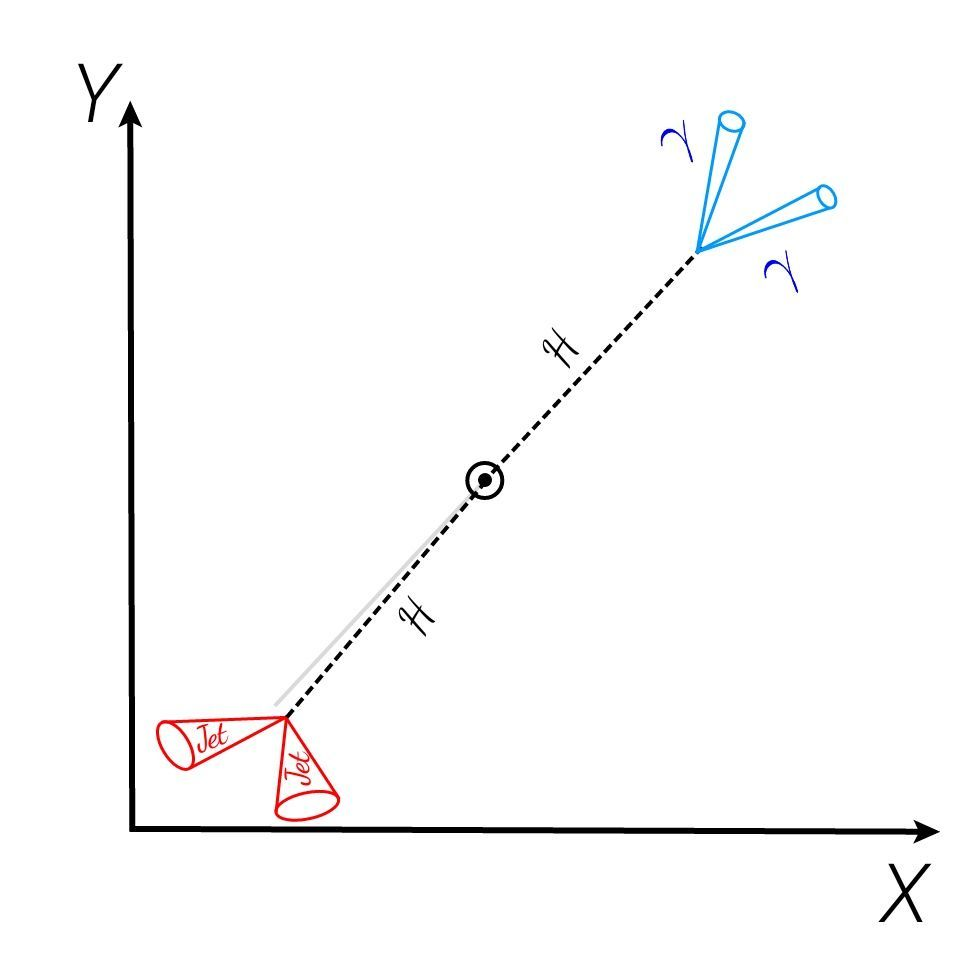
\includegraphics[width=7cm,height=7cm]{Adx/Adx4/Img/HH.png}
    \begin{tcolorbox}[colback=black!5!white,colframe=white!75!black]
    \caption{\HHyybb in the transverse plane.}
    \label{fig:Adx4:HH}
    \end{tcolorbox}

\end{figure}
\section{HH system balance}

The per-event fit uses a log-likelihood minimization to balance the HH system. Additional jets in the event are degrading the balance of the HH system significantly, making the possible gain achieved with the KF significant only in the cases of zero or one additional jet denote 0-jet and 1-jet respectively. Figure \ref{fig:Adx4:ISR} shows the Initial State Radiation (ISR) at parton level for ZH process in both qq and ggF production mode and for HH process in ggF mode. Due to the dominant ggF mode of HH production leading to large jet multiplicity, only $\sim$50\% of the events could benefit from this fit compared to ZH which is mainly initiated by quark anti-quark. In the following the likelihood fit will be defined only for 0-jet and 1-jet events.  
\begin{figure}[htbp]
    \centering
    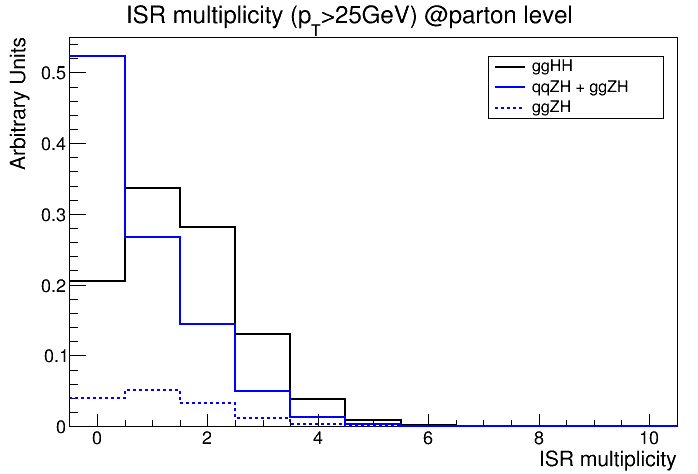
\includegraphics[width=0.5\textwidth]{Adx/Adx4/Img/isr.png}
    \begin{tcolorbox}[colback=black!5!white,colframe=white!75!black]
    \caption{Number of Initial State Radiation for qqF ZH, ggF ZH and ggF HH.}
    \label{fig:Adx4:ISR}
    \end{tcolorbox}
    
\end{figure}

\section{Likelihood}

The most general expression of the likelihood includes the 3-momenta of the 4 final states which translates into 12 inputs as free variables:
\begin{itemize}
    \item The energies of the two photons and the two $b$-jets,
    \item The pseudo-rapidities and azimutal angles of the 2 photons and 2 $b$-jets,
    \item The energy, pseudo-rapidity and azimutal angles of the additional jet (only for 1-jet event)
\end{itemize}
and implements 2 constraint terms:
\begin{itemize}
    \item The transverse momentum of the $b\bar{b}\gamma\gamma$ system is constraint to be zero with a width $\sigma_{b\bar{b}\gamma\gamma}$ obtained from simulated \HHyybb events and optimized for each events type (0-jet or 1-jet) to maximize the improvement of \mbb resolution.
    \item Assume parameters to follow Gaussian distributions.
\end{itemize}

Given the fit parameters and constraints defined above, the log-likelihood is defined as :

\begin{equation}
    \centering
    -2log(\mathcal{L}) = \sum_{i} (\frac{\Omega_i^*-\Omega_i}{\sigma_{\Omega_i}})^2 - 2log(L(p_T)) + (\frac{ \sum p_x^*-0}{\sigma_{\sigma_{b\bar{b}\gamma\gamma}}})^2 + (\frac{ \sum p_y^*-0}{\sigma_{\sigma_{b\bar{b}\gamma\gamma}}})^2.
\end{equation}

This is a product of Gaussian terms of $\Omega = (E, \eta, \phi)$ and a $p_T$-dependent jet response likelihood $L(p_T)$. The likelihood also includes a term constraining the sum over all $P_{x,y}$ momenta of the system. The energy and angular resolutions of photons are fixed to 1\% as well as the angular resolutions of the jets. Jets energy resolution is $p_T$-depend. Jet response and resolution are evaluated in the $t\bar{t}$ MC samples used to drive the $p_T$Reco function using parton level as target. Finally, this statistics is used to minimize and balance the reconstructed HH system on an event-by-event basis. It was checked that fixing the direction of the particles did not imply a loss in final resolution while it reduces significantly the computing time to converge. For that, angles are fixed in the fit to their nominal value to improve computational cost as well as to preserve the \myy distribution.  
\section{$\sigma_{b\bar{b}\gamma\gamma}$ determination}
An empirical scan is done to find the minimum value of $\sigma_{b\bar{b}\gamma\gamma}$ which correspond to the best \mbb resolution improvement. For \HHyybb, the event kinematic is changing with different \kl value as illustrated in Figure \ref{fig:chap1:HH:BSM:MHH}, thus changing in the HH system balance. Therefore, for high \kl values the event kinematic gets harder to balance and large $\sigma_{b\bar{b}\gamma\gamma}$ are favoured by the fit, thus small improvement in \mbb is expected for high \kl values. Figure \ref{fig:Adx4:Scan} shows the empirical scan of $\sigma_{b\bar{b}\gamma\gamma}$ for different \kl for both 0-jet and 1-jet. 

\begin{figure}[htbp]
   \centering
   \subfloat[0-jet][0-jet]{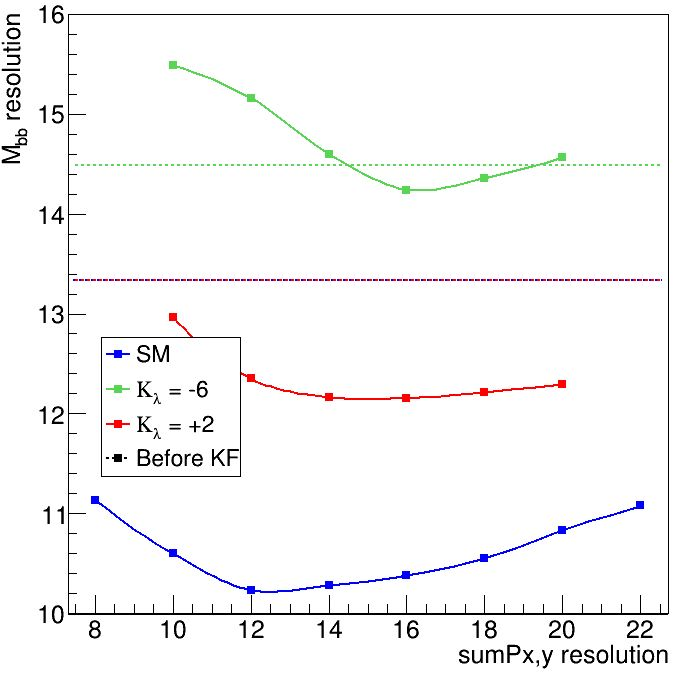
\includegraphics[width=.35\textwidth]{Adx/Adx4/Img/0JetScan.png}}
   \subfloat[1-jet][1-jet]{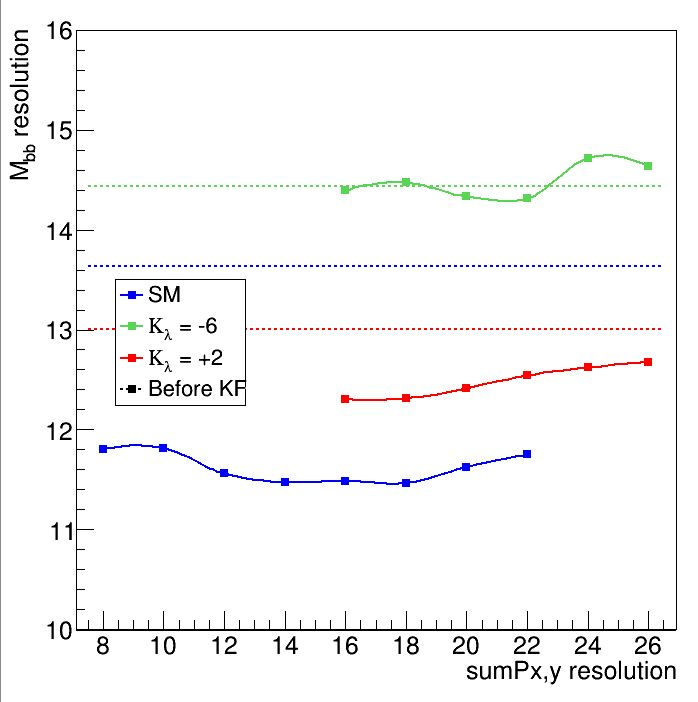
\includegraphics[width=.35\textwidth]{Adx/Adx4/Img/1JetScan.png}}
   \begin{tcolorbox}[colback=black!5!white,colframe=white!75!black]
   \caption{\mbb resolution in GeV as a function of $\sigma_{b\bar{b}\gamma\gamma}$ for (a) 0-jet and (b) 1-jet. Blue shows the scan for SM case (\kl = 1), red is BSM case of \kl = 2 and green is for \kl = -6. Lines show \mbb resolution before the kinematic fit for each case ($b$-jet calibration).}
   \label{fig:Adx4:Scan}
   \end{tcolorbox}
   
\end{figure}

For 0-jet, the maximum \mbb resolution improvement is obtained for $\sigma_{b\bar{b}\gamma\gamma}$ = 12 GeV for SM, while this value get bigger for large \kl. As expected the $\sigma_{b\bar{b}\gamma\gamma}$ is worse for 1-jet than 0-jet given the additional jet in the event. For simplicity, the optimal value of $\sigma_{b\bar{b}\gamma\gamma}$ chosen are 14 and 16 GeV for 0-jet and 1-jet respectively. This choice is motivated from the di-Higgs combination result which excludes already value of \kl less than -6.  

\section{Kinematic Fit results}

\subsection{HH system balance}
Figures \ref{fig:Adx4:HH:0Jet} and \ref{fig:Adx4:HH:1Jet} show the $p_x$ and $p_y$ of the HH system before and after the KF for both 0-jet and 1-jet events. After the KF, the HH system balance is more constrained to zero as expected and significance improvement in $p_x$ and $p_y$ is achieved. 

\begin{figure}[htbp]
   \centering
   \subfloat[$p_x$][$p_x$]{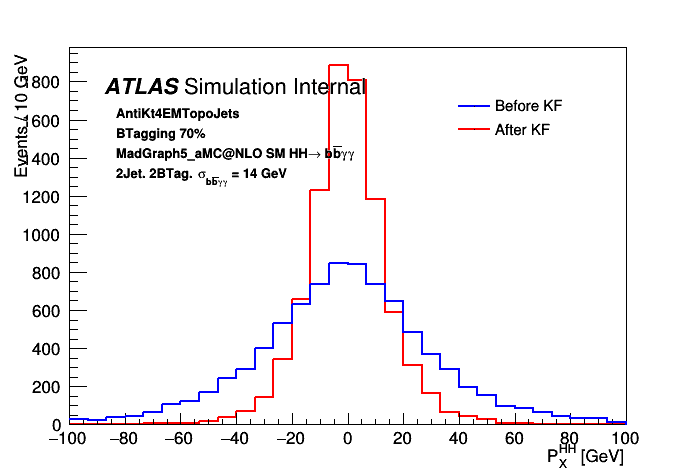
\includegraphics[width=.48\textwidth]{Adx/Adx4/Img/pxhh_KF_2Jet_AntiKt4EMTopoJets.png}}
   \subfloat[$p_y$][$p_y$]{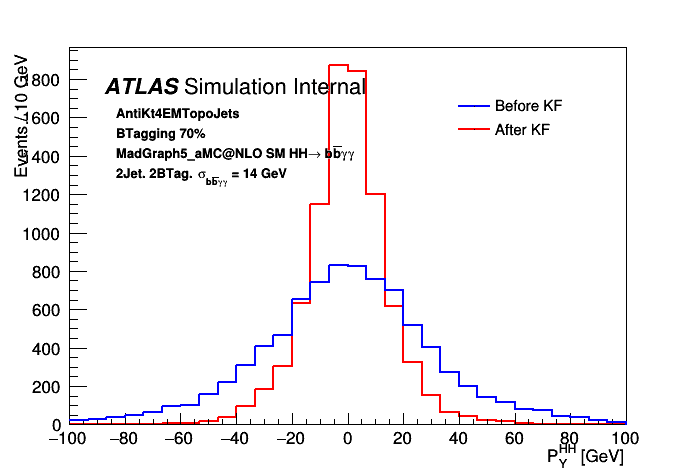
\includegraphics[width=.48\textwidth]{Adx/Adx4/Img/pyhh_KF_2Jet_AntiKt4EMTopoJets.png}}
   \begin{tcolorbox}[colback=black!5!white,colframe=white!75!black]
   \caption{$p_x$ and $p_y$ distributions of HH after (red) and before (blue) applying the kinematic fit for 0-jet events. The $\sigma_{b\bar{b}\gamma\gamma} = $ 14 GeV is used. The kinematic fit is applied on top of the $b$-jet calibration.}
   \label{fig:Adx4:HH:0Jet}
   \end{tcolorbox}
   
\end{figure}
\begin{figure}[htbp]
   \centering
   \subfloat[$p_x$][$p_x$]{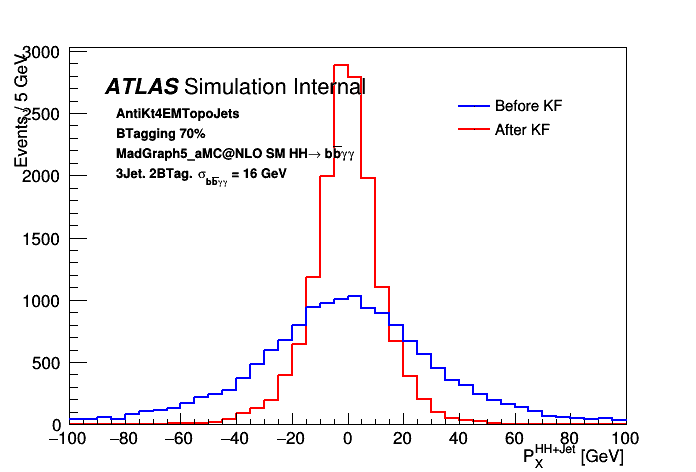
\includegraphics[width=.48\textwidth]{Adx/Adx4/Img/pxhh_KF_3Jet_AntiKt4EMTopoJets.png}}
   \subfloat[$p_y$][$p_y$]{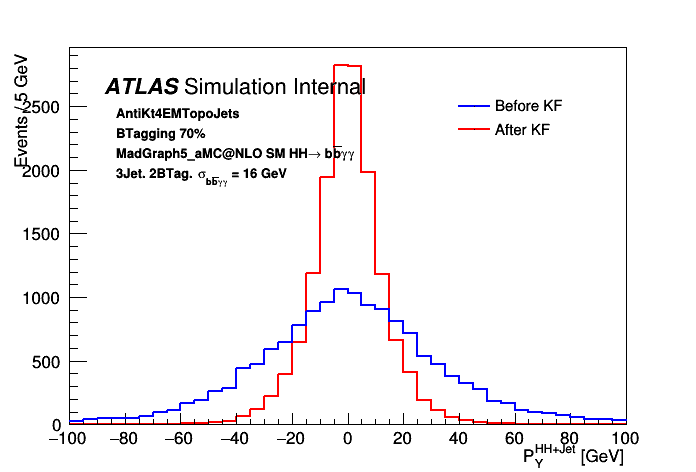
\includegraphics[width=.48\textwidth]{Adx/Adx4/Img/pyhh_KF_3Jet_AntiKt4EMTopoJets.png}}
   \begin{tcolorbox}[colback=black!5!white,colframe=white!75!black]
   \caption{$p_x$ and $p_y$ distributions of HH after (red) and before (blue) applying the kinematic fit for 1-jet events. The $\sigma_{b\bar{b}\gamma\gamma} = $ 14 GeV is used. The kinematic fit is applied on top of the $b$-jet calibration.}
   \label{fig:Adx4:HH:1Jet}
   \end{tcolorbox}
   
\end{figure}

\subsection{\mbb resolution}

Figure \ref{fig:Adx4:HH:mbb} shows the \mbb distribution after the kinematic fit for both 0-jet and 1-jet. An additional 10\% (5\%) improvement is achieved in \mbb resolution for 0-jet (1-jet) events. Figure \ref{fig:Adx4:HH:myy} shows the \myy distribution after and before the kinematic fit for both 0-jet and 1-jet: no significant change is observed as expected.
\begin{figure}[htbp]
   \centering
   \subfloat[0-jet][0-jet]{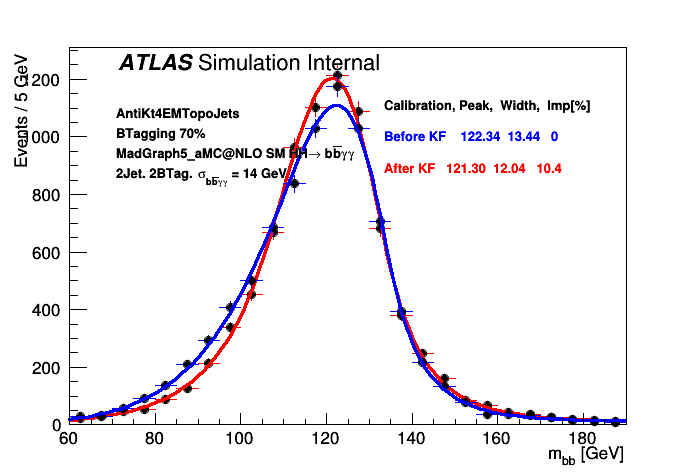
\includegraphics[width=.48\textwidth]{Adx/Adx4/Img/mbb_KF_2Jet_AntiKt4EMTopoJets.png}}
   \subfloat[1-jet][1-jet]{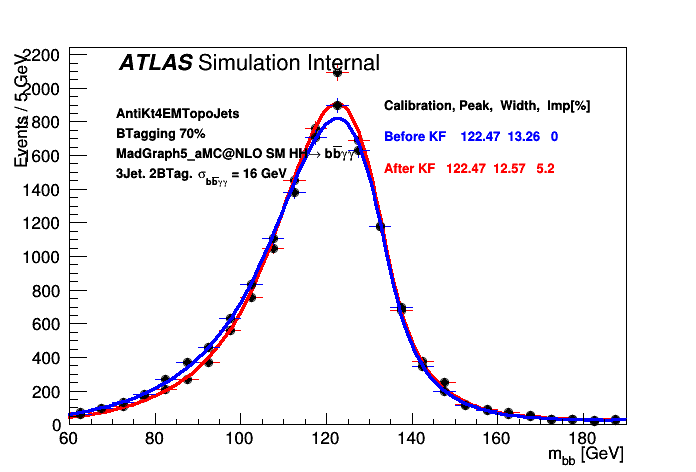
\includegraphics[width=.48\textwidth]{Adx/Adx4/Img/mbb_KF_3Jet_AntiKt4EMTopoJets.png}}
   \begin{tcolorbox}[colback=black!5!white,colframe=white!75!black]
   \caption{\mbb distributions after (red) and before (blue) applying the kinematic fit for (a) 0-jet and (b) 1-jet events. The kinematic fit is applied on top of the $b$-jet calibration.}
   \label{fig:Adx4:HH:mbb}
   \end{tcolorbox}
   
\end{figure}

\begin{figure}[htbp]
   \centering
   \subfloat[0-jet][0-jet]{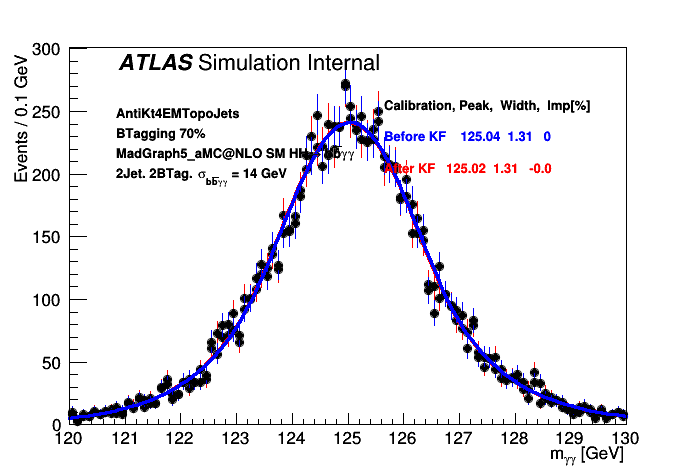
\includegraphics[width=.48\textwidth]{Adx/Adx4/Img/myy_KF_2Jet_AntiKt4EMTopoJets.png}}
   \subfloat[1-jet][1-jet]{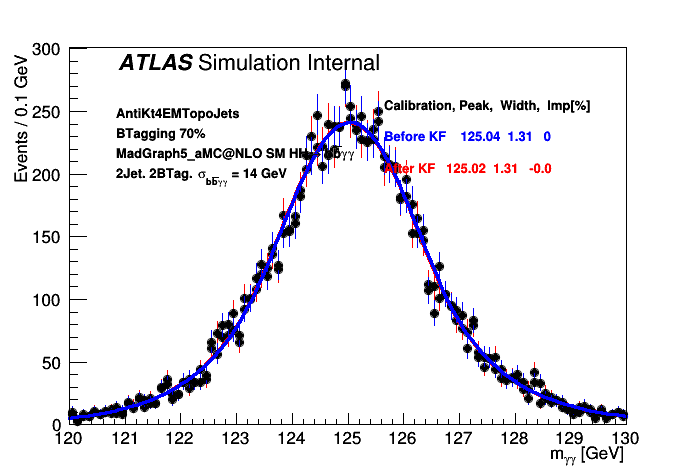
\includegraphics[width=.48\textwidth]{Adx/Adx4/Img/myy_KF_2Jet_AntiKt4EMTopoJets.png}}
   \begin{tcolorbox}[colback=black!5!white,colframe=white!75!black]
   \caption{\myy distributions after (red) and before (blue) applying the kinematic fit for (a) 0-jet and (b) 1-jet events.}
   \label{fig:Adx4:HH:myy}
   \end{tcolorbox}
   
\end{figure}


\section{Conclusion}

An additional improvement in \mbb resolution is achieved with the kinematic fit, and no changes in \myy is observed. In addition to that, no artificial peak is created in the \mbb distribution for the continuum or the $t\bar{t}$H backgrounds and an improvement in the Z peak resolution is obtained for the ZH background. The developed kinematic fit is not used in the final analysis because a bug was found in its implementation after samples production, and fixing the bug for this round would have delayed the analysis. The large jet ISR is critical for \HHyybb KF, including information about the event soft radiation in the fit is mandatory to improve its performance. The soft-term MET describes the soft radiation in the event. It could be included to improve the HH system balance. Figure \ref{fig:Adx4:HH:MET} shows the $p_x$ of the HH system for qqZH, ggZH and ggHH for different events ISR multiplicity with and without including the soft radiation. Similar $p_x$ resolution is achieved for both qq and ggF initiated process, thus the motivation to improve the KF by including soft-term MET in the likelihood. 

\begin{figure}[htbp]
   \centering
   \subfloat[ggHH][ggHH]{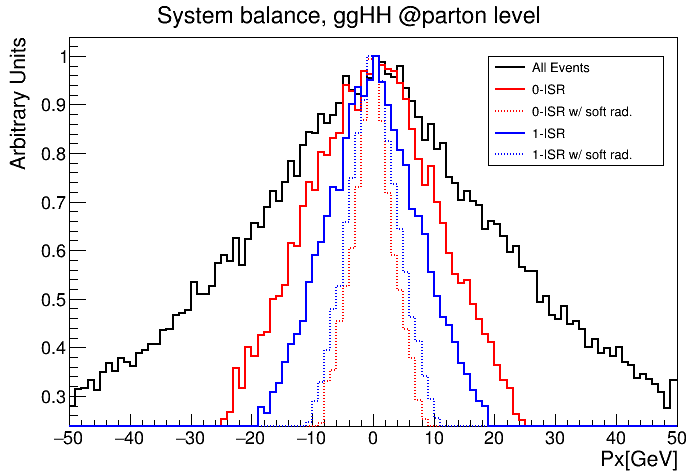
\includegraphics[width=.48\textwidth]{Adx/Adx4/Img/ggHH_px_wSoft.png}}
   \subfloat[ggZH][ggZH]{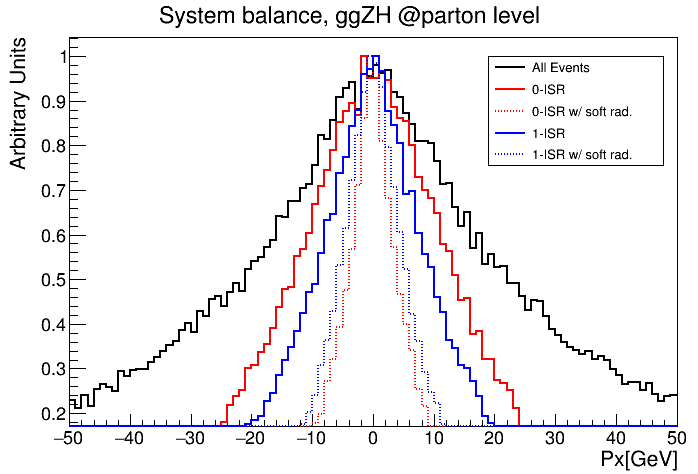
\includegraphics[width=.48\textwidth]{Adx/Adx4/Img/ggZH_px_wSoft.png}} \\
   \subfloat[qqZH][qqZH]{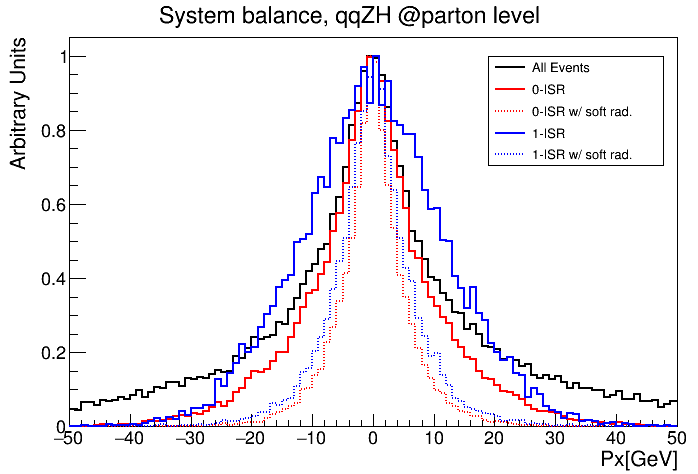
\includegraphics[width=.48\textwidth]{Adx/Adx4/Img/qqZH_px_wSoft.png}} \\
   \begin{tcolorbox}[colback=black!5!white,colframe=white!75!black]
   \caption{$p_x$ distribution for different ISR multiplicity before (solid line) and after (dashed line) including the soft radiation to compute the $p_x$ for different processes.}
   \label{fig:Adx4:HH:MET}
   \end{tcolorbox}
   
\end{figure}